\documentclass{article}

\usepackage{fullpage}
\usepackage{xcolor}
\usepackage{amsmath}
\usepackage{amssymb}
\usepackage{amsthm}
\usepackage{mathtools}
\usepackage{url}
\usepackage{latexsym}
\usepackage{paralist}


% settings for algorithm2e psuedocode style
\usepackage[procnumbered, ruled, linesnumbered, commentsnumbered, noend]{algorithm2e}
% a few parameters that are set to typeset pseudocode
\SetAlCapNameSty{textsc}
\SetProcNameSty{textsc}
\SetProcArgSty{textsc}

%style for pseudocode comments
\newcommand\mycommfont[1]{\footnotesize\ttfamily\textcolor{darkgray}{#1}}
\SetCommentSty{mycommfont}

% used for formatting graphs
\usepackage{tikz}
\usetikzlibrary{arrows}

\theoremstyle{definition}
\newtheorem{problem}{Problem}
\newtheorem*{solution}{Solution}
\newtheorem*{resources}{Resources}


\newcommand{\honor}{\noindent \textbf{Aggie Honor Statement: }On my honor as an Aggie, I have neither
  given nor received any unauthorized aid on any portion of the academic work included in this assignment.
}


\newcommand{\checklist}{\noindent\textbf{Checklist:}
Did you...
\begin{compactenum}
\item abide by the Aggie Honor Code?
\item solve all problems?
\item start a new page for each problem?
\item show your work clearly?
\item type your solution?
\item submit a PDF to eCampus?
\end{compactenum}
}

\newcommand{\problemset}[1]{\begin{center}\textbf{Problem Set #1}\end{center}}
\newcommand{\duedate}[1]{\begin{quote}\textbf{Due: #1} on eCampus (\url{ecampus.tamu.edu}). \\You must show your work in order to recieve credit.\end{quote}}
\newcommand{\mysectionnumber}[0]{503}

\title{CSCE 222: Discrete Structures for Computing\\Section \mysectionnumber\\Fall 2016}
\author{Joseph Martinsen}

\begin{document}

\maketitle

\problemset{4}

\duedate{25 September 2016 (Sunday) before 11:59 p.m.}

\bigskip

% Sets and Set Operations
\begin{problem} (30 points)\\
Consider the sets $P = (A-B)-C$ and $Q = (A-C) - (B-C)$.\\
Determine which relationship ($\subseteq,=,\supseteq$) holds between the two sets $P$ and $Q$.\\
Your answer will be either $P \subseteq Q$, or $P = Q$, or $P \supseteq Q$.\\
Justify your answer three ways by
  \begin{enumerate}
    \item drawing the Venn diagram,
    \item constructing the membership table, and
    \item proving it (using set identities with set builder notation).
  \end{enumerate}
  \end{problem}

\begin{solution}\
  \begin{enumerate}
    \item Drawing the Venn diagram
      \begin{figure}[h]
        \centering
        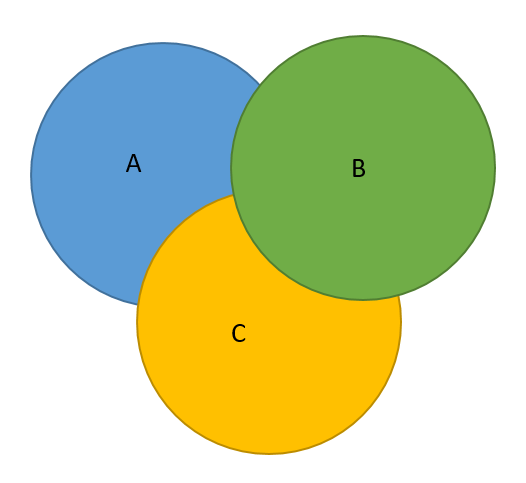
\includegraphics[scale=0.4]{VennDiagP01.png}
        \caption{Venn Diagram of both sets }
      \end{figure}

    \item Constructing the membership table
      \begin{center}
       \begin{tabular}{||c|c|c||c|c|c|c|c|}
         \hline
         $A$ & $B$ & $C$ & $A-B$ & $A-C$ & $B-C$ & $(A-B)-C$ & $(A-C)-(B-C)$\\ [0.5ex]
         \hline\hline
         0 & 0 & 0 & 0 & 0 & 0 & 0 & 0 \\
         \hline
         0 & 0 & 1 & 0 & 0 & 0 & 0 & 0 \\
         \hline
         0 & 1 & 0 & 0 & 0 & 1 & 0 & 0 \\
         \hline
         0 & 1 & 1 & 0 & 0 & 0 & 0 & 0 \\
         \hline
         1 & 0 & 0 & 1 & 1 & 0 & 1 & 1 \\
         \hline
         1 & 0 & 1 & 1 & 0 & 0 & 0 & 0 \\
         \hline
         1 & 1 & 0 & 0 & 1 & 1 & 0 & 0 \\
         \hline
         1 & 1 & 1 & 0 & 0 & 0 & 0 & 0 \\
         \hline
      \end{tabular} \\ \ \\
      $(A-B)-C = (A-C) - (B-C)$ because they have the same truth values \\
      $\therefore   P = Q$
    \end{center}

    \item Using set identities with set builder notation.
      \begin{equation*}
        \begin{aligned}
          A-B            & = \{x \mid x \in A \wedge x \notin B \} \\
          (A-B) - C      & = \{x \mid x \in (A-B) \wedge x \notin C\} \\
                         & = \{x \mid x \in A \wedge x \notin B \wedge x \notin C \} \\ \ \\
          (A-C)          & = \{x \mid x \in A \wedge x \notin C \} \\
          (B-C)          & = \{x \mid x \in B \wedge x \notin C \} \\
          (A-C) - (B-C)  & = \{x \mid x \in (A-C) \wedge x \notin (B-C) \} \\
                         & = \{x \mid x \in A \wedge x \notin B \wedge x \notin C \} \\
          (A-C)-(B-C)    & = (A-B)-C = \{x \mid x \in A \wedge x \notin B \wedge x \notin C \}\\
          \therefore   P & = Q
        \end{aligned}
      \end{equation*}
  \end{enumerate}

\end{solution}

\newpage

% Sets and Set Operations
\begin{problem} (20 points)\\
Show that if $A$, $B$, and $C$ are sets, then $|A \cup B \cup C| = |A| + |B| + |C| - |A \cap B| - |A \cap C| - |B \cap C| + |A \cap B \cap C|$.
\end{problem}

\begin{solution}
  \begin{equation*}
    \begin{aligned}
      |A \cup B \cup C| & = |A| \cup |B \cup C| \\
      & = |A| + |B \cup C| - |A \cap |B \cup C|| \\
      & = |A| + |B + C - B \cap C| - ||A \cap B| \cup |A \cap C|| \\
      & = |A| + |B| + |C| - |B \cap C| - ||A \cap B| + |A \cap C| - |A \cap B| \cap |A \cap C|| \\
      & = |A| + |B| + |C| - |A \cap B| - |A \cap C| - |B \cap C| + |A \cap B \cap C|
    \end{aligned}
  \end{equation*}
\end{solution}
\newpage



\bigskip
\honor

\bigskip
\checklist
\end{document}
